\chapter{Implementation details}
\label{chap: id}

This Chapter speaks about the implementation specifics of D3driver. This proof of concept demonstrates the possibility of execution of the solution idea that has been proposed in this thesis. 

\section{Overview of D3driver}
D3driver is a productivity bot that is uploaded as a custom app in Microsoft Teams tool. It is aimed at providing a feasible solution to teams that involve multiple domains while designing a product. It aids documenting design related decisions during a conversation between members from different domains. The team members discuss questions, answers, ideas, concepts, solutions, alternatives and decisions in their group chats. Since, decisions play a crucial role in product development, D3driver's features aid team members to track specifically design decisions document all the design decisions for later data retrieval. 

The installation guidelines of D3driver is first explained. Later, the usage is also briefly re-explained to get more familiar with the bot. Finally, each the development of each feature/functionality is explained along with their code snippets for better and clear understanding of the implementation of D3driver. The source code for this implementation is based on the boilerplate code available from the official Microsoft's online guide called Bot builder samples\footnote{https://github.com/microsoft/BotBuilder-Samples}

\section{D3driver Installation} 
The app package after uploading in MS Teams, D3driver's scope is within channels. The option `Add to team' can be selected to install the bot in the required channel. Once the D3driver is installed in a channel it sets up a messaging extension under the conversation area and a D3driver tab in the tab section as shown in the Figure \ref{fig:meandtabformarking}. 

\begin{figure}
\centering
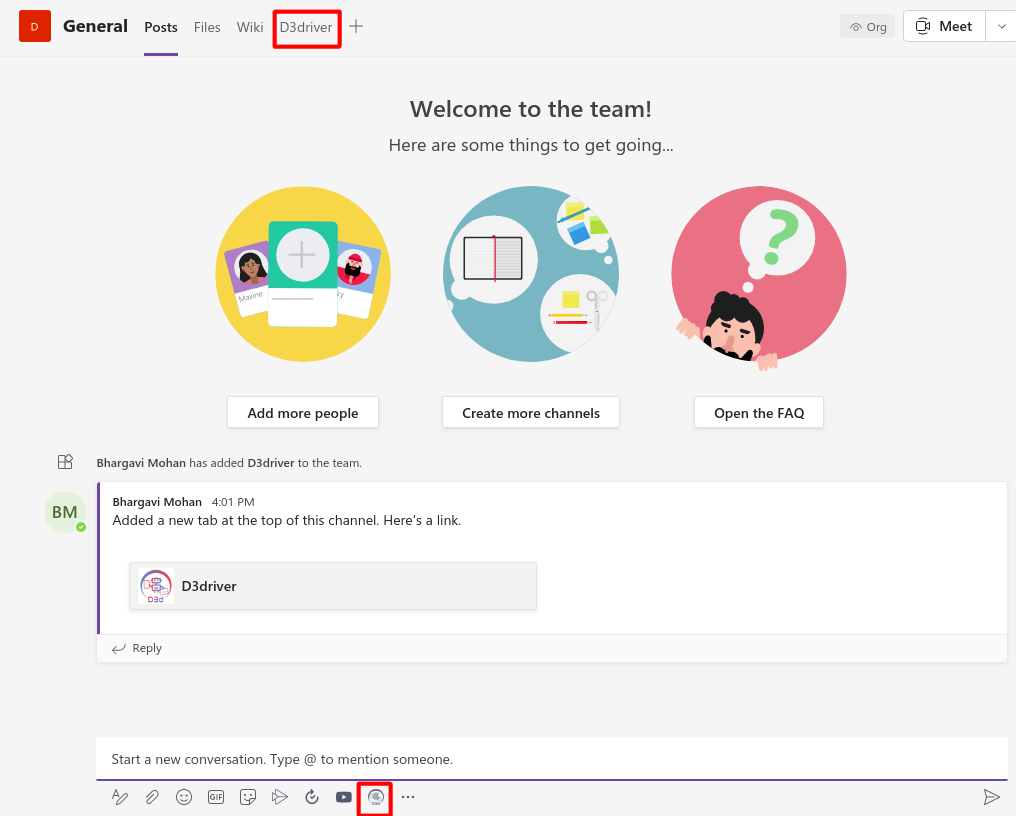
\includegraphics[width=0.8\linewidth]{figures/meandtabformarking}
\caption{Message extension icon and D3driver tab}
\captionsetup{justification=centering}
\label{fig:meandtabformarking}
\end{figure}

\subsection{Usage}
\begin{itemize}
\item Firstly, a channel should be initialized. This means a team should first select one of the three phases in V-model for accessing design decision cards. The three phases will have 3 different decision cards hence a decision card in a channel depends upon the type of initialization. The command to initialize the channel is made available in the command list. The user has to invoke the bot by typing '@D3driver' in the compose message area and the list of commands will appear. The command \texttt{init} is used to initialize the channel 

\item Once the \texttt{init} command is used to invoke the bot, D3driver replies to the channel with an initial card. A user is required to select the appropriate design phase suitable to a particular channel. 

\item Depending on the choice, the decision cards can be accessed either by invoking the bot followed by the command --- \texttt{Create card} or by hitting the messaging extension. The easiest and fastest way is to just hit the messaging extension. 

\item The different decision cards for architectural phase, design/conceptual phase and implementation phase are shown in Figures \ref{fig:fdd}, \ref{fig:dce} and \ref{fig:sw} respectively.

\item When users decide to decommission a channel, another command in the list \texttt{del} is available. By doing so, all the decisions discussed will be erased from the database. The users can choose to save the data to their local system before using \texttt{del} command by using the button "Export as PDF". It enables the members to save the entire D3driver tab as a PDF file. The filename will be in $<$channel name$>$\_$<$vphase name$>$ format. 

\end{itemize}

\section{D3driver and its components}
Firstly, when a user sends any message by invoking the bot, the control goes to the main python file \texttt{app.py} as shown in Listing \ref{lst:app.py}. It has a method called \texttt{messages()} that keeps snooping on any incoming messages and gives control to the object \texttt{BOT} of the class \newline
\texttt{TeamsMessagingExtensionsActionPreviewBot}.

\begin{lstlisting}[caption={app.py},label={lst:app.py},language=python]

BOT = TeamsMessagingExtensionsActionPreviewBot()
async def messages(req: Request) -> Response:
    # Main bot message handler.

    if "application/json" in req.headers["Content-Type"]:
        body = await req.json()
    else:
        return Response(status=HTTPStatus.UNSUPPORTED_MEDIA_TYPE)

    activity = Activity().deserialize(body)

    auth_header = req.headers["Authorization"] if "Authorization" in req.headers else ""

    invoke_response = await ADAPTER.process_activity(


        activity, auth_header, BOT.on_turn
    )

    if invoke_response:
        return json_response(
            data=invoke_response.body, status=invoke_response.status
        )

    return Response(status=HTTPStatus.OK)
\end{lstlisting}

This way, on any incoming message the control is transferred to the class. There are four important methods inside the class. 1) A method that takes control when the incoming message \texttt{init} 2) A method that takes control when the incoming message is \texttt{del} 3) A method that takes control when the messaging extension is invoked to access a decision card 4) A method that takes control when the submit button of the decision card is hit. This means that there is one method for each of the three commands and one method for submitting the decision card(this method is explained in the end, after decision cards are also discussed). These methods are explained in detail along with the details of the commands in the next section .
\subsection{Commands}
 There are 3 useful commands that come handy while using this bot. \texttt{init} , \texttt{del} and \texttt{Create card} are shown in Figure \ref{fig:commands}. The result of typing "@D3driver" followed by either of the commands is discussed one-by-one in sub sections \ref{init} , \ref{del}, \ref{me}.



\subsubsection{\textbf{init}}
\label{init}
When a channel needs to be initialized, the control jumps to the method  \texttt{on\_message\_activity()} of class \texttt{TeamsMessagingExtensionsActionPreviewBot}. The following code snippet in Listing \ref{lst:initmethod} explains how this request is handled. The variable \texttt{text\_command} checks if the \texttt{D3driverinitcommand} is assigned the value \texttt{init}, if all the conditions meet, then the V-model phase selection card is posted in the channel. The card offers the channel members to choose the type of initialization that is required for their channel as shown in the Figure \ref{fig:vphasecard}. 

\begin{lstlisting}[caption={init command handling},label={lst:initmethod},language=python]
elif text_command == D3driverinitcommand:
                        #vphase = 'Model-based'
                result = database.find_channel_exists(channel_id)
                if(len(result) == 0):
                    card = create_vphase_card_editor()
                    task_info = TaskModuleTaskInfo(
                    card=card, height=450, title="Design decision card", width=500
                        )
                    message = MessageFactory.attachment(card)
                    response_id = await turn_context.send_activity(message)
\end{lstlisting}


\begin{figure}[h]
\centering
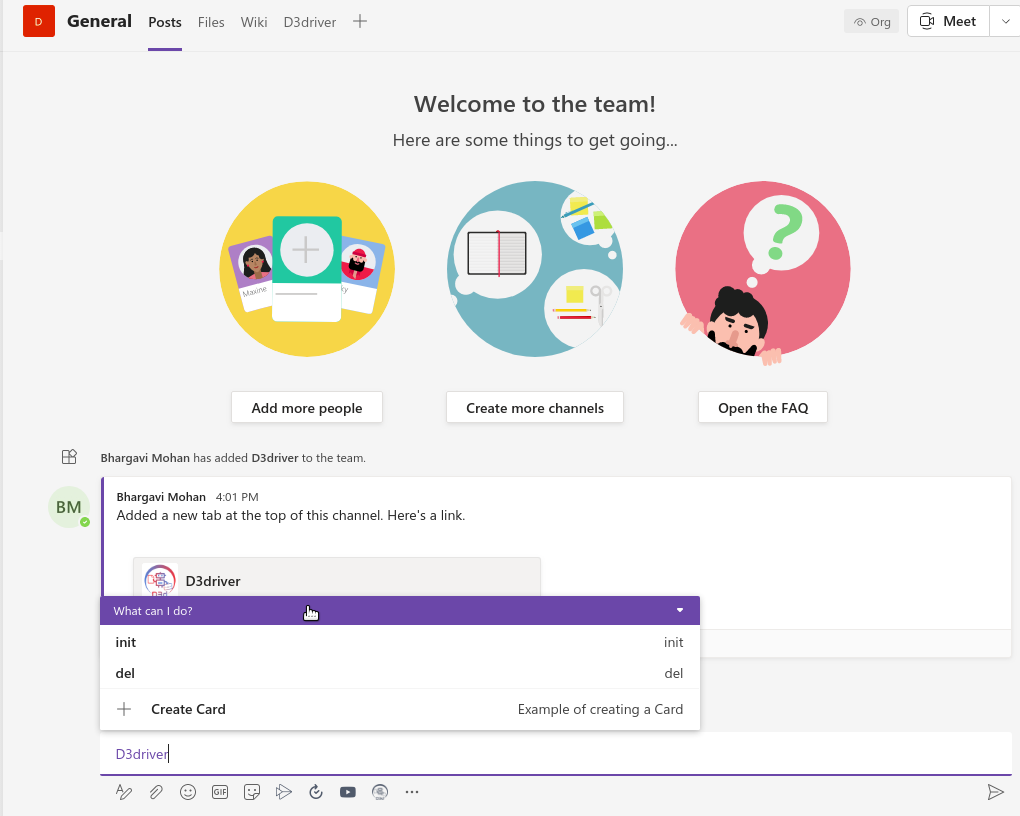
\includegraphics[width=0.7\linewidth]{figures/commands}
\captionsetup{justification=centering}
\caption{Commands}
\label{fig:commands}
\end{figure}
 
 
\begin{figure}[h]
\centering
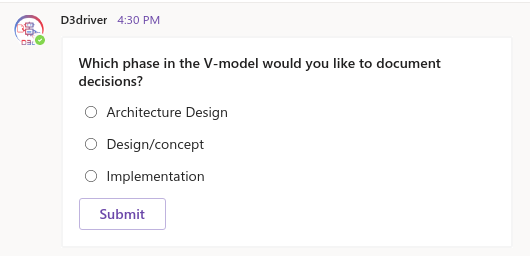
\includegraphics[width=0.7\linewidth]{figures/vphasecard}
\captionsetup{justification=centering}
\caption{V-model phase selection card}
\label{fig:vphasecard}
\end{figure} 


The Listing \ref{lst:vphasecard} shows how the V-model phase card is created. It defined the \texttt{action} section and indicates that an action has to be taken when the choices are submitted. The \texttt{body} section defined some of the text formatting definitions and the \texttt{choices} that lists the available choices that are part the card. 

\begin{lstlisting}[caption={V-model phase card},label={lst:vphasecard},language=python]
def create_vphase_card_editor(
    user_text: str = None,
    is_multi_select: bool = False,
    option1: str = None,
    option2: str = None,
    option3: str = None,
) -> Attachment:
    return CardFactory.adaptive_card(
        {
            "actions": [
                {
                    "data": {"submitLocation": "messagingExtensionFetchTask", "type" : "vmodelinit"},
                    "title": "Submit",
                    "type": "Action.Submit",
                }
            ],

                "body": [
                    {
                    "text": "Which phase in the V-model would you like to document decisions?",
                    "type": "TextBlock",
                    "weight": "bolder",
                    "wrap": True,
                },
                    {
                        "choices": [
                            {
                                "title": "Architecture Design",
                                "value": "Architecture Design"
                            },
                            {
                                "title": "Design/concept",
                                "value": "Design/concept"
                            },
                            {
                                "title": "Implementation",
                                "value": "Implementation"
                            }   
                        ],
			"id": "Choices",
                    	"isMultiSelect": is_multi_select,
                    	"style": "expanded",
                    	"type": "Input.ChoiceSet",
                    },
                ],
		        "type": "AdaptiveCard",
            	"version": "1.0",
            }
    )
\end{lstlisting}


\subsubsection{\textbf{del}}
\label{del}

This command is used in two scenarios. One is when the users decide that they no more need D3driver in their channel, it can be uninstalled by deleting the data present. An other likely scenario is when the users want to re-initialize the channel because they decide to use a different V-model phase for their project. If the team members would want to discuss a different set of design decisions, then users have to use the command \texttt{del} to reset their type of initialization. The control of the program is given to a different block in the method \texttt{on\_message\_activity()} as shown in Listing \ref{lst:delmethod}. The variable \texttt{text\_command} checks if the \texttt{D3driverdelcommand} is assigned the value \texttt{del}. If the conditions are met, then the records of this channel and decisions are all deleted from the database. A message is posted on the channel informing the successful deletion.
 
\begin{lstlisting}[caption={del command handling},label={lst:delmethod},language=python]
elif text_command == D3driverdelcommand:
                database.delete_channel(channel_id)
                database.delete_decision(channel_id)
                reply = MessageFactory.text(
                "This channel is no more initialized. All the design decsions(if discussed) has been deleted from the database. Plase click on 'Export to PDF' button in D3driver tab to save all the data to your local device. To re-initialize the channel, please enter "
                "the init command"
                )
                await turn_context.send_activity(reply)
\end{lstlisting}


\subsubsection{\textbf{Create card command / click on Messaging extension}}
\label{me}
The \texttt{Create card} command triggers the messaging extension that is configured for D3driver which means choosing the \texttt{Create card} command and clicking on the D3driver's messaging extension has the exact same effect. The control is transferred to the same method in the code and D3driver reacts to both the events in the same way. There needs to be a little background knowledge on how it is possible to incorporate messaging extension service in the D3driver.  

The Bot Framework SDK provides developers all the necessary tools, \textbf{adaptive cards}, messaging schema and communication protocols. To be able to use the SDK, a developer has to register the bot in the bot framework. The developer needs to provide some information during the registration like a name for the bot, optional endpoint etc. A Bot ID and password is generated at the end of the registration which will be required later. The bot registration of D3driver is shown in the Figure \ref{fig:botreg} and this is how the messaging extension is set up for D3driver.

\begin{figure}[h]
\centering
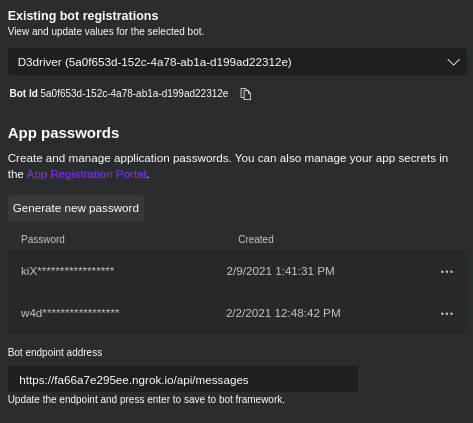
\includegraphics[width=0.8\linewidth]{figures/botreg}
\captionsetup{justification=centering}
\caption{Bot registration}
\label{fig:botreg}
\end{figure}


In general, an action based messaging extension provides the team members with a popup. This popup can either gather information from the members or display a piece of information to the members. The gathered information is then inserted into the channel. The purpose of messaging extension in D3driver is to access decision cards and gather design decisions to be documented when any user inputs the decisions in the intended text-box area. Likewise, all the members of the channel can access decision cards to exchange design decision information and this is enabled by having the messaging extension configured.  After the user hits submit button, the web service hosted by the bot framework is returned by posting the decision card to the channel. 

Observe the Listing \ref{lst:fetchtask}. The control of the program is now transferred to a different method i,e. to
\texttt{on\_teams\_messaging\_extension\_fetch\_task()}. This method examines which type of initialization a particular channel has and sends appropriate cards accordingly. The variable \texttt{result} is checked if it holds the value ``Architecture
Design" or ``Design/Concept" or ``Implementation" and three different cards namely ``create\_ad\_adaptive\_card\_editor()" or ``create\_dc\_adaptive\_card\_editor()" or ``create\_imp\_adaptive\_card\_editor()" are posted to the channel depending on the value of \texttt{result}. The method also performs certain database operations to check if the channel is already initialized, if yes, relevant message is posted on the channel else requested card will be rendered. 

\begin{lstlisting}[caption={messaging\_extension\_action\_preview\_bot.py},label={lst:fetchtask},language=python]
 async def on_teams_messaging_extension_fetch_task(
        self, turn_context: TurnContext, action: MessagingExtensionAction
    ) -> MessagingExtensionActionResponse:
        if turn_context.activity.conversation.conversation_type != 'personal':
            channel_id = turn_context.activity.channel_data['channel']['id']
            conversation_id = turn_context.activity.conversation.id #to distinguish 'Generals' of different teams
            channel_name = turn_context.activity.conversation.name
            if channel_name is None:
                channel_name = 'General'
            result = database.find_channel_exists(channel_id)
            if(len(result) == 1):
                if(result[0]["channel"]["vphase"] == 'Architecture Design'):
                    card = create_ad_adaptive_card_editor()
                    task_info = TaskModuleTaskInfo(
                        card=card, height=450, title="Design decision card", width=500
                    )
                    continue_response = TaskModuleContinueResponse(value=task_info)
                    return MessagingExtensionActionResponse(task=continue_response)
                elif(result[0]["channel"]["vphase"] == 'Design/concept'):
                    card = create_dc_adaptive_card_editor()
                    task_info = TaskModuleTaskInfo(
                        card=card, height=450, title="Design decision card", width=500
                    )
                    continue_response = TaskModuleContinueResponse(value=task_info)
                    return MessagingExtensionActionResponse(task=continue_response)
                elif(result[0]["channel"]["vphase"] == 'Implementation'):
                    card = create_imp_adaptive_card_editor()
                    task_info = TaskModuleTaskInfo(
                        card=card, height=450, title="Design decision card", width=500
                    )
                    continue_response = TaskModuleContinueResponse(value=task_info)
                    return MessagingExtensionActionResponse(task=continue_response)
            else: 
                reply = MessageFactory.text(
                "Hi there! Please initialize your channel before accessing the cards by using the init command." 
                )
                await turn_context.send_activity(reply)
        else:
            reply = MessageFactory.text(
            "***D3driver*** is pleased to help you with decision cards in your required channels. Please access the bot using the default commands in any channel. ***Happy Documenting!***"
            )
            await turn_context.send_activity(reply)
\end{lstlisting}

Some of the important inbuilt classes and their object instances of the Bot framework SDK that is operating in Listing \ref{lst:fetchtask} is explained in the following sub sections for deeper understanding.
\raggedbottom
\paragraph{Turncontext}
By passing the class \texttt{TurnContext} as argument in the function calls as shown in \ref{lst:fetchtask}, it means new instance of the TurnContext class can be created. An object of the class \texttt{TurnContext} is imported from the package \texttt{botbuilder-core} in the bot framework. This object is helpful to get the specific context during the bot's turn for processing inputs or triggering events. The context enables the developers to access all the necessary metadata and values to handle activities that are upcoming. Furthermore, another class \texttt{BotAdapter} handles the context object creation and other internal operations like authentication, sending and receiving activities from Bot service. The \texttt{TurnContext} has a couple of constructors and various properties and methods to perform specific actions.

\paragraph{MessagingExtensionAction}
This class specifies the action brought by the messaging extension. It extends a class \texttt{TaskModulerequest}. This class calls upon the request payload. \newline \texttt{MessagingExtensionAction} offers various parameters to access the user input data, user context, command ID, command context, message payload etc. It also has properties to get or set bot activity preview, get or set the ID of the command assigned by bot and gets or set message content sent as part of the command request etc. 
			
\paragraph{MessagingExtensionActionResponse}
This class returns a response to the messaging extension action. As seen in Listing \ref{lst:fetchtask} the class accepts a parameter \texttt{task} that returns the JSON for the Adaptive card to be rendered in the task module.

This marks the end of available commands in D3driver and how the corresponding function methods are called depending on the type of commands. Next, the three types of decision cards depending on the three types of initialization are discussed in the following section.

\subsection{Decision cards}
The decision cards in D3driver depends on the type of initialization. If the channel is initialized with ``Architectural design" then the card shown in Figure \ref{fig:ad} is popped up when \texttt{Create card} command is used or when messaging extension is clicked.

\begin{figure}[h]
\centering
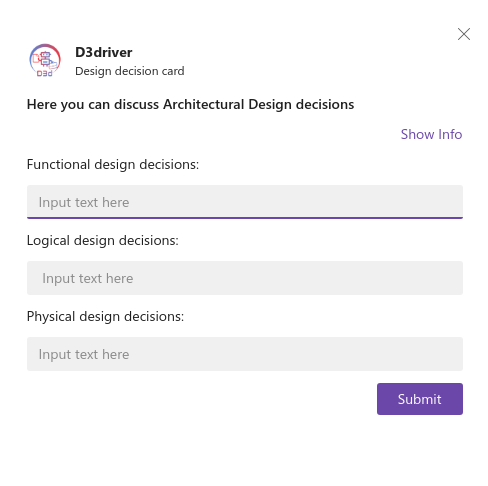
\includegraphics[width=0.6\linewidth]{figures/ad}
\captionsetup{justification=centering}
\caption{Architectural design decision card}
\label{fig:ad}
\end{figure}

The method \texttt{create\_ad\_adaptive\_card\_editor} seen in Listing \ref{lst:adcard} is called when \texttt{Create card} command is used or when messaging extension is clicked. It returns an attachment i.e. the adaptive card of type architectural design. The attachment will contain the card with a suitable `contentType'. A TypeError is caused if the card arguments are not python dicts. The adaptive cards are written in JSON format as seen in Listings \ref{lst:adcard}, \ref{lst:dccard} and \ref{lst:impcard}. The JSON has different parameters such as the field \texttt{actions} to define what has to be done when the submit button is clicked, the field \texttt{body} that defines the heading of the card, content of the sub headings and text-box areas and alignement, the field \texttt{Container} in the body indicates the meaning of each type of decision. The \texttt{Container} element introduces a toggle button called ``Show info" and ``Hide info" in UI of the decision card as seen in Figure \ref{fig:ad}. The values of the fields deliver the styling and other formatting features to appear in the adaptive cards to make them look elegant and flawless.


\begin{lstlisting}[caption={Architectural design card},label={lst:adcard},language=python]
def create_ad_adaptive_card_editor(
    user_text1: str = None,
    user_text2: str = None,
    user_text3: str = None,
) -> Attachment:
    return CardFactory.adaptive_card(
        {
            "actions": [
                {
                    "data": {"submitLocation": "messagingExtensionFetchTask"},
                    "title": "Submit",
                    "type": "Action.Submit",
                }
            ],
            "body": [
                {
                    "text": "Here you can discuss Architectural Design decisions",
                    "type": "TextBlock",
                    "weight": "bolder",
                },
                {
            "type": "ColumnSet",
            "columns": [
                {
                    "type": "Column",
                    "selectAction": {
                        "type": "Action.ToggleVisibility",
                        "targetElements": [
                            "cardContent4",
                            "showInfo",
                            "hideInfo"
                        ]
                    },
                    "verticalContentAlignment": "Center",
                    "items": [
                        {
                            "type": "TextBlock",
                            "id": "showInfo",
                            "horizontalAlignment": "Right",
                            "color": "Accent",
                            "text": "Show Info",
                            "wrap": True
                        },
                        {
                            "type": "TextBlock",
                            "id": "hideInfo",
                            "horizontalAlignment": "Right",
                            "color": "Accent",
                            "text": "Hide Info",
                            "wrap": True,
                            "isVisible": False
                        }
                    ],
                    "width": 1
                }
            ]
        },
        {
            "type": "Container",
            "id": "cardContent4",
            "isVisible": False,
            "items": [
                {
                    "type": "Container",
                    "items": [
                        {
                            "type": "TextBlock",
                            "text": "* ***Functional design decisions:*** Decisions related to functions describe functionality of the system under consideration independant of the solution.",
                            "isSubtle": True,
                            "wrap": True
                        },
                        {
                            "type": "TextBlock",
                            "text": "* ***Logical design decisions:*** Decisions related to logical architecture describes a possible implementation of the functions with defined solution principles.",
                            "isSubtle": True,
                            "wrap": True
                        },
                        {
                            "type": "TextBlock",
                            "text": "* ***Physical design decisions:*** Decisions related to the physical element describes the actual implementation, e.g. technical elements with part numbers, concrete source code, etc.",
                            "isSubtle": True,
                            "wrap": True
                        }
                    ]
                }
            ]
        },
                {"type": "TextBlock", "text": "Functional design decisions:"},
                {
                    "id": "Question1",
                    "placeholder": "Input text here",
                    "type": "Input.Text",
                    "value": user_text1,
                    "isRequired": True,
                    "errorMessage": "Any one feild is required"
                },
                
                {"type": "TextBlock", "text": "Logical design decisions:"},
                {
                    "id": "Question2",
                    "placeholder": " Input text here",
                    "type": "Input.Text",
                    "value": user_text2,
                },
                {"type": "TextBlock", "text": "Physical design decisions:"},
                {
                    "id": "Question3",
                    "placeholder": "Input text here",
                    "type": "Input.Text",
                    "value": user_text3,
                },  
            ],
            "type": "AdaptiveCard",
            "version": "1.0",
        }
    )
\end{lstlisting}



If the channel is initialized with ``Design/concept", then the card shown in Figure \ref{fig:dc} shows up and the card is developed as shown in Listing \ref{lst:dccard}. Note the descriptions of what type of decisions can be discussed using this decision template to guide the users.



\begin{lstlisting} [caption={Design/conceptual card card},label={lst:dccard},language=python]
def create_dc_adaptive_card_editor(
    user_text1: str = None,
    user_text2: str = None,
    user_text3: str = None,
) -> Attachment:
    return CardFactory.adaptive_card(
        {
            "actions": [
                {
                    "data": {"submitLocation": "messagingExtensionFetchTask"},
                    "title": "Submit",
                    "type": "Action.Submit",
                }
            ],
            "body": [
                {
                    "text": "Here you can discuss Design/conceptual decisions",
                    "type": "TextBlock",
                    "weight": "bolder",
                },
                {
            "type": "ColumnSet",
            "columns": [
                {
                    "type": "Column",
                    "selectAction": {
                        "type": "Action.ToggleVisibility",
                        "targetElements": [
                            "cardContent4",
                            "showInfo",
                            "hideInfo"
                        ]
                    },
                    "verticalContentAlignment": "Center",
                    "items": [
                        {
                            "type": "TextBlock",
                            "id": "showInfo",
                            "horizontalAlignment": "Right",
                            "color": "Accent",
                            "text": "Show Info",
                            "wrap": True
                        },
                        {
                            "type": "TextBlock",
                            "id": "hideInfo",
                            "horizontalAlignment": "Right",
                            "color": "Accent",
                            "text": "Hide Info",
                            "wrap": True,
                            "isVisible": False
                        }
                    ],
                    "width": 1
                }
            ]
        },
        {
            "type": "Container",
            "id": "cardContent4",
            "isVisible": False,
            "items": [
                {
                    "type": "Container",
                    "items": [
                        {
                            "type": "TextBlock",
                            "text": "* ***Design definition decisions:*** Decisions related to technology management,design objectives and design definition strategy, including the need for and requirements of any enabling systems, products, or services.",
                            "isSubtle": True,
                            "wrap": True
                        },
                        {
                            "type": "TextBlock",
                            "text": "* ***Design characteristics & Enablers decisions:*** Decisions related to  design characteristics for the architectural entities that ensures that the design characteristics are feasible. Design enablers such as models (physical and analytical), design heuristics, etc. are decided.",
                            "isSubtle": True,
                            "wrap": True
                        },
                        {
                            "type": "TextBlock",
                            "text": "* ***Design Alternatives decisions:*** Decisions related to assessing options for the system element to be developed using selection criteria. The most appropriate alternatives decision is made to develop the system element.",
                            "isSubtle": True,
                            "wrap": True
                        }
                    ]
                }
            ]
        },
                {"type": "TextBlock", "text": "Design definition decisions:"},
                {
                    "id": "Question1",
                    "placeholder": "Input text here",
                    "type": "Input.Text",
                    "value": user_text1,
                },
                {"type": "TextBlock", "text": "Design characteristics & Enablers decisions:"},
                {
                    "id": "Question2",
                    "placeholder": "Input text here",
                    "type": "Input.Text",
                    "value": user_text2,
                },
                {"type": "TextBlock", "text": "Design Alternatives decisions:"},
                {
                    "id": "Question3",
                    "placeholder": "Input text here",
                    "type": "Input.Text",
                    "value": user_text3,
                },  
            ],
            "type": "AdaptiveCard",
            "version": "1.0",
        }
    )
\end{lstlisting}

\begin{figure}[h]
\centering
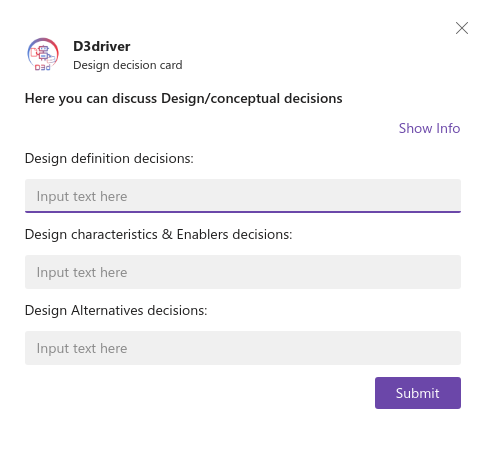
\includegraphics[width=0.7\linewidth]{figures/dc}
\captionsetup{justification=centering}
\caption{Design/concept decision card}
\label{fig:dc}
\end{figure}

If the channel is initialized with "Implementation", then the card in Figure \ref{fig:imp} appears to the users. The card is developed as shown in Listing \ref{lst:impcard}. Please observe the meanings of each decision type described to guide the users.
\begin{figure}[h]
\centering
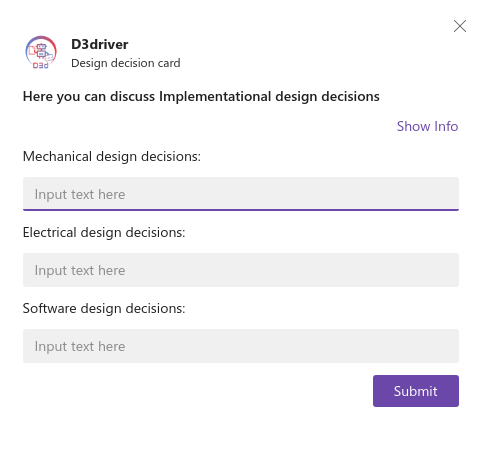
\includegraphics[width=0.6\linewidth]{figures/imp}
\captionsetup{justification=centering}
\caption{Implementation decision card}
\label{fig:imp}
\end{figure}

\begin{lstlisting} [caption={Implementation card},label={lst:impcard},language=python]
def create_imp_adaptive_card_editor(
    user_text1: str = None,
    user_text2: str = None,
    user_text3: str = None,
) -> Attachment:
    return CardFactory.adaptive_card(
        {
            "actions": [
                {
                    "data": {"submitLocation": "messagingExtensionFetchTask"},
                    "title": "Submit",
                    "type": "Action.Submit",
                }
            ],
            "body": [
                {
                    "text": "Here you can discuss Implementational design decisions",
                    "type": "TextBlock",
                    "weight": "bolder",
                },
                {
            "type": "ColumnSet",
            "columns": [
                {
                    "type": "Column",
                    "selectAction": {
                        "type": "Action.ToggleVisibility",
                        "targetElements": [
                            "cardContent4",
                            "showInfo",
                            "hideInfo"
                        ]
                    },
                    "verticalContentAlignment": "Center",
                    "items": [
                        {
                            "type": "TextBlock",
                            "id": "showInfo",
                            "horizontalAlignment": "Right",
                            "color": "Accent",
                            "text": "Show Info",
                            "wrap": True
                        },
                        {
                            "type": "TextBlock",
                            "id": "hideInfo",
                            "horizontalAlignment": "Right",
                            "color": "Accent",
                            "text": "Hide Info",
                            "wrap": True,
                            "isVisible": False
                        }
                    ],
                    "width": 1
                }
            ]
        },
        {
            "type": "Container",
            "id": "cardContent4",
            "isVisible": False,
            "items": [
                {
                    "type": "Container",
                    "items": [
                        {
                            "type": "TextBlock",
                            "text": "* ***Mechanical design decisions:*** Decisions related to mechanics like displacement, velocity, acceleration, force , torque etc.",
                            "isSubtle": True,
                            "wrap": True
                        },
                         {
                            "type": "TextBlock",
                            "text": "* ***Electrical design decisions:*** Decisions related to electronics like electric variables, voltage, current, electric field strength etc.",
                            "isSubtle": True,
                            "wrap": True
                        },
                         {
                            "type": "TextBlock",
                            "text": "* ***Software design decisions:*** Decisions related to digital information process like logical operations, algorithms, database etc.",
                            "isSubtle": True,
                            "wrap": True
                        }
                    ]
                }
            ]
        },
                {"type": "TextBlock", "text": "Mechanical design decisions:"},
                {
                    "id": "Question1",
                    "placeholder": "Input text here",
                    "type": "Input.Text",
                    "value": user_text1,
                },
                {"type": "TextBlock", "text": "Electrical design decisions:"},
                {
                    "id": "Question2",
                    "placeholder": "Input text here",
                    "type": "Input.Text",
                    "value": user_text2,
                },
                {"type": "TextBlock", "text": "Software design decisions:"},
                {
                    "id": "Question3",
                    "placeholder": "Input text here",
                    "type": "Input.Text",
                    "value": user_text3,
                },  
            ],
            "type": "AdaptiveCard",
            "version": "1.0",
        }
    )
\end{lstlisting}


This ends the discussion about the three types of cards that are made available in D3driver to discuss and document design decisions. The following sub section deals with the action taken by D3driver when the ``submit" button is clicked in each of the decision cards. The same action is taken in all three cases and is addressed as follows.

\subsubsection{\textbf{Submit button}} 
When the users insert their discussion topic in the cards and hits the submit button, the control is transferred to a method that handles this event. The four important methods of the class \texttt{TeamsMessagingExtensionsActionPreviewBot} were listed earlier. This section describes the forth method \texttt{on\_teams\_messaging\_extension\_submit\_action()} that performs two tasks. It captures the decision type, decision maker's name, date and the design decision topic and makes a database store operation to save all the information of the user that is about to submit the card. Secondly, the card is posted on the channel. The card is called ``Preview card" and this way the sender is making his decision public by clicking on submit button. The ``preview card" can be visualized in the Figures \ref{fig:fdd},\ref{fig:dce} and \ref{fig:sw}. One card from each type of initialization is depicted. The method also handles a scenario when users do not type anything and hits submit, an error message is posted. The ``preview card" is developed as shown in Listing \ref{lst:pcard}. 

\begin{lstlisting}[caption={Submit button handling},label={lst:submit},language=python]
async def on_teams_messaging_extension_submit_action(  # pylint: disable=unused-argument
        self, turn_context: TurnContext, action: MessagingExtensionAction
    ) -> MessagingExtensionActionResponse:

        channel_id = turn_context.activity.channel_data['channel']['id']
        year = str(turn_context.activity.local_timestamp.year)
        month = str(turn_context.activity.local_timestamp.month)
        day = str(turn_context.activity.local_timestamp.day)
        decisiondate = year + "-" + month + "-" + day
        channel_name = turn_context._activity.conversation.name
        if channel_name is None:
            channel_name = 'General'
        result = database.find_channel_exists(channel_id)
        if(result[0]["channel"]["vphase"] == 'Architecture Design'):
            a="Functional design decision"
            b="Logical design decision"
            c="Physical design decision"
        elif(result[0]["channel"]["vphase"] == 'Design/concept'):
            a="Design definition desisions"
            b="Design characteristics and enablers desicions"
            c="Design alterantives decisions"
        elif(result[0]["channel"]["vphase"] == 'Implementation'):
            a="Mechanical design decisions"
            b="Electrical design decisions"
            c="Software design decisions"


        user_text1 = action.data["Question1"],
        user_text2 = action.data["Question2"],
        user_text3 = action.data["Question3"],

        if(user_text1[0] == ''):
            a = ''
        if(user_text2[0] == ''):
            b = ''
        if(user_text3[0] == ''):
            c = ''
   
        memberid = turn_context._activity.from_property.name
        card = create_adaptive_card_preview(
             user_text1[0],
             user_text2[0],
             user_text3[0],
             a,
             b,
             c,
             memberid,
        )

        # db entries
        if(result[0]["channel"]["vphase"] == 'Architecture Design'):
            database.insert_decision(channel_id,channel_name,memberid,decisiondate,
            a,user_text1,b,user_text2,c,user_text3)
        elif(result[0]["channel"]["vphase"] == 'Design/concept'):
            database.insert_decision(channel_id,channel_name,memberid,decisiondate,
            a,user_text1,b,user_text2,c,user_text3)
        elif(result[0]["channel"]["vphase"] == 'Implementation'):
            database.insert_decision(channel_id,channel_name,memberid,decisiondate,
            a,user_text1,b,user_text2,c,user_text3)
        

        if (user_text1[0] or user_text2[0] or user_text3[0] != ''):
            message = MessageFactory.attachment(card)
            await turn_context.send_activity(message)
    
            return MessagingExtensionActionResponse()
        else:  
            reply = MessageFactory.text(
            "Error. No decision made"
            )
            await turn_context.send_activity(reply) 
\end{lstlisting}

\begin{figure}[h]
\centering
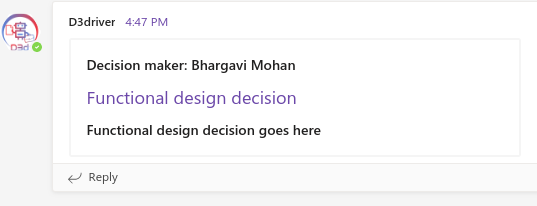
\includegraphics[width=0.7\linewidth]{figures/fdd}
\captionsetup{justification=centering}
\caption{Functional design decision posted on channel}
\label{fig:fdd}
\end{figure}

\begin{figure}[h]
\centering
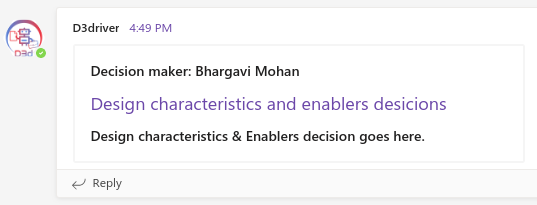
\includegraphics[width=0.7\linewidth]{figures/dce}
\captionsetup{justification=centering}
\caption{Design characteristics and enablers decision posted on channel}
\label{fig:dce}
\end{figure}

\begin{figure}[h]
\centering
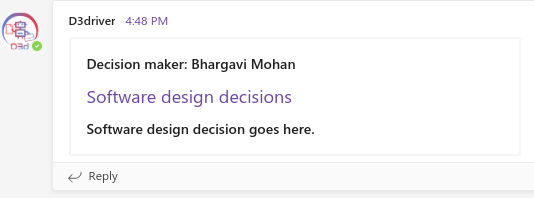
\includegraphics[width=0.7\linewidth]{figures/sw}
\captionsetup{justification=centering}
\caption{Software design decision posted on channel}
\label{fig:sw}
\end{figure}





\begin{lstlisting}[caption={Preview card},label={lst:pcard},language=python]
def create_adaptive_card_preview(
    user_text1: str = None,
    user_text2: str = None,
    user_text3: str = None,
    a: str = None,
    b: str = None,
    c: str = None,
    memberid: str = None,
) -> Attachment:
    return CardFactory.adaptive_card(
        {
            "body": [
                {
                    "text": "Decision maker: {}".format(memberid),
                    "type": "TextBlock",
                    "weight": "bolder",
                },
                {
                    "text": "{}".format(a), 
                    "type": "TextBlock", 
                    "id": "Question1",
                    "color": "Accent",
                    "size": "Large"
                },
                {
                    "text": "{}".format(user_text1), 
                    "type": "TextBlock", 
                    "id": "Question1",
                    "weight": "bolder"
                },


                {
                    "text": "{}".format(b),
                    "type": "TextBlock", 
                    "id": "Question2",
                    "color": "Accent",
                    "size": "Large"
                },
                {
                    "text": "{}".format(user_text2), 
                    "type": "TextBlock", 
                    "id": "Question1",
                    "weight": "bolder"
                },
                { 
                    "text": "{}".format(c), 
                    "type": "TextBlock", 
                    "id": "Question3",
                    "color": "Accent",
                    "size": "Large"
                },
                {
                    "text": "{}".format(user_text3), 
                    "type": "TextBlock", 
                    "id": "Question1",
                    "weight": "bolder"
                },

            ],
            "type": "AdaptiveCard",
            "version": "1.0",
        }
    )
\end{lstlisting}

\section{D3driver Tab}
There are two types of tabs in Microsoft teams. 1) Static tabs and 2) Configurable tabs. Configurable tab is the focus in this thesis. It lets one to set the content of the tab dynamically each time the 
bot is added to a channel. It is nothing but a web-based HTML page generated inside a teams configurable tab. The content URL must be set properly to see a working configurable tab.(The endpoint URL can be submitted while the bot registration explained in \ref{me})

D3driver installs a configurable tab upon bot installation and the welcome page is previewed before the tab is installed as shown in Figure \ref{fig:welcomepageintab}. Once the tab is saved to a channel, all the channel specific data appears in the configured tab. The tab serves like a dashboard that displays all the design decisions discussed along with its other parameters in a team. Every channel will has its own D3driver tab and the design decisions, channel initialization type and other important information present in a tab will pertain to its respective channel. The tab will additionally have a search box, sort button and a button to export the tab as a PDF and a button to view the meta data in JSON format as shown in Figure \ref{fig:d3dtabnew}. 

\begin{figure}[h]
\centering
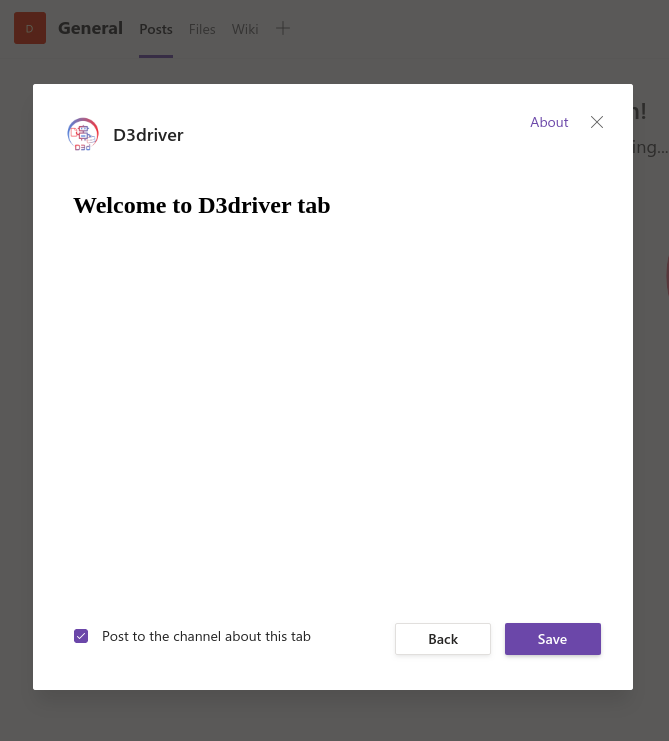
\includegraphics[width=0.6\linewidth]{figures/welcomepageintab}
\captionsetup{justification=centering}
\caption{Welcome tab}
\label{fig:welcomepageintab}
\end{figure}

\subsection{Ngrok}

The way the content is published in the tab is by using an \texttt{ngrok} tunnel. Using \texttt{ngrok}, the local endpoint is exposed to the internet hence making the HTML content available publicly. The \texttt{ngrok} providing public URL in terminal can be seen in Figure \ref{fig:ngrok}. The command to expose the local end point is right below. 

\begin{lstlisting}[language=bash]
  $ ngrok http -host-header=rewrite 3978
\end{lstlisting}

\begin{figure}[h]
\centering
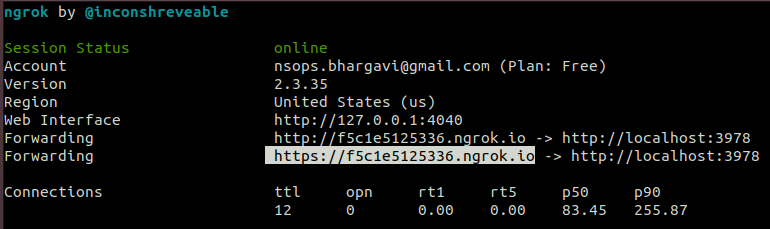
\includegraphics[width=0.7\linewidth]{figures/ngrok}
\captionsetup{justification=centering}
\caption{Ngrok endpoint}
\label{fig:ngrok}
\end{figure}


\subsection{Jinja}

Furthermore, for the purpose of templating HTML, Jinja is used. It is a web template tool for python coding. This well known template engine is responsible for populating all the mark up, source code, database records in the D3driver tab. According to the Listing \ref{lst:dash}, a page is rendered by applying \texttt{@aiohttp\_jinja2.template()} decorator to the web-handler. The method \texttt{dashboard} returns a jnja2 context. The decorator now presents the context as the web response. The python list variables \texttt{response\_obj\_tables} and \texttt{response\_obj\_decisions} capture the required data records from the database to pass it on the to the desired HTML file(dashboard.html).

\begin{figure}[h]
\centering
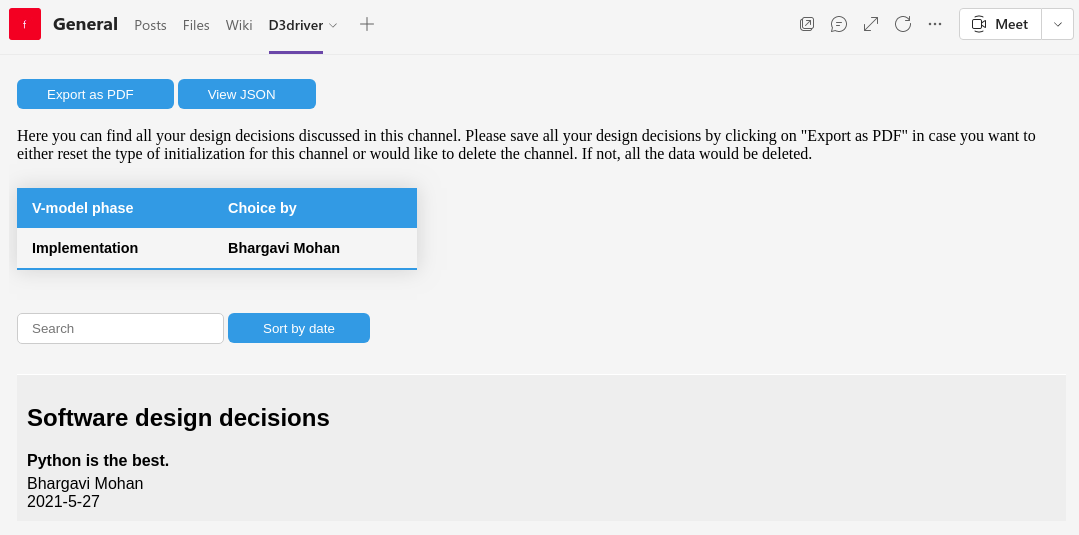
\includegraphics[width=0.9\linewidth]{figures/d3dtabnew}
\caption{D3driver tab installed in a channel}
\label{fig:d3dtabnew}
\end{figure}

\begin{lstlisting}[caption={Dashboard method},label={lst:dash},language=python]
@aiohttp_jinja2.template("dashboard.html")
async def dashboard(request):  
    try:
        param = request._rel_url.query_string
        param = param.strip('channelid=')
        response_obj_tables = database.get_channel_details(param)
        response_obj_decisions = database.get_all_decisions(param)
        ## rErroreturn a success json response with status code 200 i.e. 'OK'
        return {"decisions_list": response_obj_decisions,"tables_list":response_obj_tables}
    except Exception as e:
        ## Bad path where 
\end{lstlisting}


\subsection{AIOHTTP}

A small web server is created using \texttt{aiohttp} to support the functionality of viewing the meta data of any channel. The meta data is the raw data that is fetched from the database. The meta data is present in the JSON format. Upon click of ``View JSON" in D3driver tab, a user is redirected to their default browser to view and further work with it to edit or copy to the local system. A request handler accepts \texttt{request} as its only argument and returns the JSON data in response as shown in Listing \ref{json}.

\begin{lstlisting}[caption=View JSON button, language=python,label=json]
async def jsonreply(request): 
    try:
        param = request._rel_url.query_string
        param = param.strip('channelid=')
        response_obj_tables = database.get_channel_details(param)
        response_obj_decisions = database.get_all_decisions(param)
        return web.json_response({"decisions_list": response_obj_decisions,"tables_list":response_obj_tables})
    except Exception as e:
        return web.json_response({"error": e})
\end{lstlisting}


\subsection{JavaScript}
Two scripts have been used for the functionality of search box, sort button and export button. The library \texttt{list.js} has been used for search and date sort functions. For the export button, html2pdf javascript library has been used. A sample javascript is shown in Listing \ref{pdfjs} to observe how the PDF download script works. 

\begin{lstlisting}[language=java,caption=PDF download script,label=pdfjs]
<script>
  window.onload = function () {
    document.getElementById("download")
        .addEventListener("click", () => {
            const invoice = this.document.getElementById("invoice");
            console.log(invoice);
            console.log(window);
            var opt = {
                margin: 1,
                filename: "{{ tables_list.name | safe}}_{{ tables_list.vphase | safe}}",
                image: { type: 'jpeg', quality: 0.98 },
                html2canvas: { scale: 2 },
                jsPDF: { unit: 'in', format: 'letter', orientation: 'portrait' }
            };
            html2pdf().from(invoice).set(opt).save();
        })
}

</script>
\end{lstlisting}

\section{Database structure}
The storage for D3driver implementation is document oriented database. The data is stored as python dictionary in TinyDB. TinyDB makes use of the Python JSON module hence query to TinyDB fetches JSON data in return. TinyDB extends its support in creation of DB tables. The data modeling in tables is as same shown in Listing \ref{lst:datamodel}. Every record in the dictionary uses the name of the table as \textbf{key} and documents dictionary as \textbf{value}. Therefore, every record is stored as a \textbf{key-value} pair. The dictionary of documents contain document IDs as keys and the documents as values.

\begin{lstlisting}[caption={Data in TinyDB tables},label={lst:datamodel},language=python]
{
    'table1': {
        0: {document...},
        1: {document...},
    },
    'table2': {
        ...
    }
}...
\end{lstlisting}

For D3driver's implementation, two such tables are used. 
\begin{enumerate}
\item \textbf{\texttt{channelstable}--- } This table stores the list of all the initialized channels. It stores other important data as shown in Listing \ref{lst:Initializedchannelsanddata}. It represents one entry in the table. The \texttt{channelid} is a unique string of characters that is assigned to each channel. The \texttt{name} is the name of the channel. \texttt{vphase} is the type of initialization of that channel. \texttt{memebername} is the member who initialized the channel to \texttt{vphase} value. \texttt{date} represents the day on which the channel was initialized.
\begin{lstlisting}[caption={Initialized channels data},label={lst:Initializedchannelsanddata},language=python]
    "Initializedchannelsanddata": {
        "1": {
            "channel": {
                "channelid": "19:5642f28c1510444d9af14304ce7ce158@thread.tacv2",
                "name": "bottest",
                "vphase": "Design/concept",
                "membername": "Bhargavi Mohan",
                "date": "2021-3-10"
            }
        }
\end{lstlisting}
\item \textbf{\texttt{decisionstable}---} This table stores all the design decisions of every initialized channel. The Listing \ref{lst:des} shows a single record of this table. The \texttt{channelid} is a unique string of characters that is assigned to each channel. The \texttt{name} is the name of the channel. \texttt{membername} represents the decision maker's name. \texttt{date} represent the day on which a particular decision has been made. \texttt{decisionname\_a} , \texttt{decisionname\_b} and \texttt{decisionname\_c} corresponds the name of design decisions. This depends once again on the type of initialization of the channel. Since the channel's name is "bottest" and it's type of initialization is "\textbf{Design/concept}" - \texttt{vphase} values in Listing \ref{lst:Initializedchannelsanddata}. Hence the \texttt{decisionname\_a} , \texttt{decisionname\_b} and \texttt{decisionname\_c} would be \textbf{Design definition decisions} , \textbf{Design characteristics \& Enablers decisions} and \textbf{Design Alternatives decisions} respectively.
In the example shown in Listing \ref{lst:des}, only decision pertaining to \textbf{Design characteristics and enablers desicions} has been made, hence there is an entry against \texttt{decisionname\_b}
The records with the key names \texttt{decision\_a}, \texttt{decision\_b} and \texttt{decision\_c} will be paired with their respective values which is the actual decision topic. In the below example, \texttt{decision\_b} has some value tagged to it.

\begin{lstlisting}[caption={Design decisions table},label={lst:des},language=python]
   "Designdecisions": {
           "1": {
               "decisions": {
                   "channelid": "19:5642f28c1510444d9af14304ce7ce158@thread.tacv2",
                   "name": "bottest",
                   "membername": "Bhargavi Mohan",
                   "date": "2021-3-10",
                   "decisionname_a": "",
                   "decision_a": "",
                   "decisionname_b": "Design characteristics and enablers desicions",
                   "decision_b": "This is a place where Design characteristics and enablers desicions will be discussed",
                   "decisionname_c": "",
                   "decision_c": ""
               }
           }
\end{lstlisting}
\end{enumerate}

\section{Sequential workflow}
The sequence diagrams are a well known way of demonstrating the interactions and operations in a process. It also depicts the order of interactions or messages sent and received. 

The 3 sequence diagrams can be observed in Figure \ref{fig:initseq},  \ref{fig:create cardseq} and \ref{fig:delseq}. These basically represent the sequence of actions,reactions and exchange of messages between different functions. The figures show the sequential workflow of what happens when users invoke the bot by using the three basic commands of D3driver. The content in the rectangular boxes depicts the file names and the messages on the arrow depicts what is the action taking place. The vertical lines are called lifelines and the arrows represent asynchronous messages and replies. 



\begin{figure}[h]
\centering
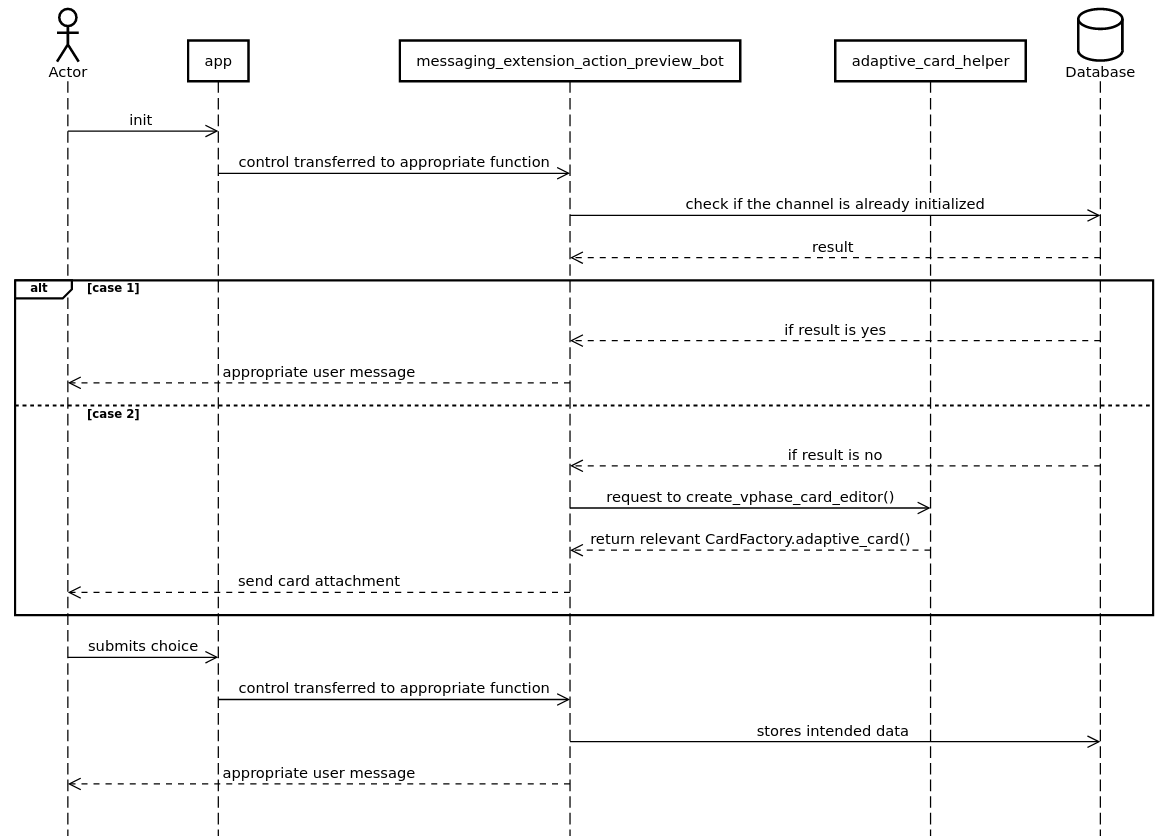
\includegraphics[width=1.1\linewidth]{figures/initseq}
\captionsetup{justification=centering}
\caption{@D3driver init}
\label{fig:initseq}
\end{figure}

In Figure \ref{fig:initseq}, the rectangular big box named ``alt" represents that there is a condition being checked. In Figure \ref{fig:create cardseq}, the big rectangular box represents that the event can happen in a loop until the user wishes to.


\begin{figure}[h]
\centering
\includegraphics[width=1.1\linewidth]{"figures/create cardseq"}
\captionsetup{justification=centering}
\caption{Create card}
\label{fig:create cardseq}
\end{figure}

\begin{figure}[h]
\centering
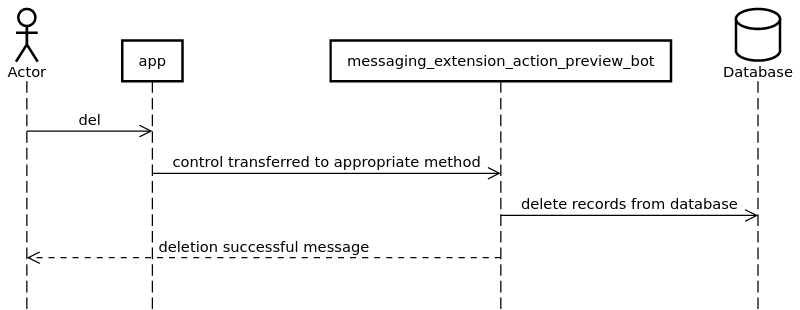
\includegraphics[width=0.9\linewidth]{figures/delseq}
\captionsetup{justification=centering}
\caption{@D3driver del}
\label{fig:delseq}
\end{figure}



\section{Manifest schema}
All the apps available in MS teams app store has to define an app manifest file. This file is a compressed file of one JSON file named as \texttt{manifest.json}, and two PNG versions of colored bot icon and an outlined bot icon of 192*192 pixels. In order to be able to upload a custom bot, the developer should prepare a zipped package of all the three. \textbf{\textit{Appstudio}}\footnote{https://microsoft.github.io/botframework-solutions/clients-and-channels/tutorials/enable-teams/4-create-app-manifest/} is already available in the MS teams app store, using which, one can easily create and edit the application manifest.

The manifest JSON file is the description of how the bot should be incorporated into Microsoft teams tool. This JSON should abide by the standard schema\footnote{https://developer.microsoft.com/en-us/json-schemas/teams/v1.8/MicrosoftTeams.schema.json} define by Microsoft. The file provides various options for attributes in its JSON body. The attributes in the JSON leads to its applicable sources such as Microsoft BOT ID, BOT password(that is generated during bot registration), a configuration URL to any static/configurable tabs. It is in this file the developer mentions if the bot should install a messaging extension , have configurable tabs , have default commands etc. There are other mandatory fields in the JSON body that should have valid values. Only when all the required fields are given the right values, the custom app(bot) can be uploaded and can be used in Microsoft teams. The app manifest of D3driver can be observed in Listing \ref{lst:manifest}. Observe the D3driver bot ID, bot full description, configuration URL that renders the D3driver tab, messaging extension configured and the scopes in which the bot is allowed to be added. 


\begin{lstlisting}[caption={Manifest file},label={lst:manifest},language=python]
{
  "$schema": "https://developer.microsoft.com/en-us/json-schemas/teams/v1.8/
  MicrosoftTeams.schema.json",
  "manifestVersion": "1.8",
  "version": "1.0",
  "id": "5a0f653d-152c-4a78-ab1a-d199ad22312e",
  "packageName": "com.microsoft.teams.samples",
  "developer": {
    "name": "UPB - Bhargavi Mohan",
    "websiteUrl": "https://dev.botframework.com",
    "privacyUrl": "https://privacy.microsoft.com",
    "termsOfUseUrl": "https://www.microsoft.com/en-us/legal/intellectualproperty/copyright/
    default.aspx"
  },
  "icons": {
    "color": "icon-color.png",
    "outline": "icon-outline.png"
  },
  "name": {
    "short": "D3driver",
    "full": "Design Decision Document driver"
  },
  "description": {
    "short": "Bot that aids documenting design decisions",
    "full": "D3driver drives the design decision documentation in the easiest way possible. This bot is exclusively designed to be used in a Mechatronics team. The design phase is an integral step in systems engineering domain. In an inter-disciplinary team, the design stage during the lifecycle of a product is extended across different phases of V-model and hence the design decisions are made throughout architectural design phase , conceptual design phase and even during the implementation phase. All these design decisions and decision makers should be distinguished from regualar or unimportant discussions that happen within a team and put together for later quick access and that is exactly what D3driver assists the users with. D3driver installs a messaging extension and a tab. The messaging extension is to access decision cards where user can choose from which phase of the V-model does the user want to document the design decisions. The tab serves like a dashboard that displays all the design decisions discusssed in a team."
  },
  "accentColor": "#FFFFFF",
  "configurableTabs": [
    {
      "configurationUrl": "https://f5c1e5125336.ngrok.io/config",
      "canUpdateConfiguration": true,
      "scopes": [
        "team"
      ],
      "context": [
        "channelTab"
      ]
    }
  ],
  "bots": [
    {
      "botId": "5a0f653d-152c-4a78-ab1a-d199ad22312e",
      "scopes": [
        "personal",
        "team"
      ],
      "commandLists": [
        {
          "scopes": [
            "team"
          ],
          "commands": [
            {
              "title": "init",
              "description": "init"
            },
            {
              "title": "del",
              "description": "del"
            }
          ]
        }
      ],
      "supportsFiles": false,
      "isNotificationOnly": false
    }
  ],
  "composeExtensions": [
    {
      "botId": "5a0f653d-152c-4a78-ab1a-d199ad22312e",
      "canUpdateConfiguration": false,
      "commands": [
        {
          "id": "createWithPreview",
          "type": "action",
          "title": "Create Card",
          "description": "Example of creating a Card",
          "initialRun": false,
          "fetchTask": true,
          "context": [
            "commandBox",
            "compose",
            "message"
          ],
          "parameters": [
            {
              "name": "param",
              "title": "param",
              "description": ""
            }
          ]
        }
      ]
    }
  ],
  "permissions": [
    "identity",
    "messageTeamMembers"
  ],
  "validDomains": [
  "7b22dd51bc42.ngrok.io",
  "*.cdnjs.cloudflare.com",
	"static2.sharepointonline.com", 
	"secure.aadcdn.microsoftonline-p.com", 
	"code.jquery.com", 
	"statics.teams.microsoft.com", 
	"*.microsoftonline.com", 
	"ajax.googleapis.com",
	"*.bing.com", 
	"*.google.com",
  	"*.statics.teams.cdn.office.net"
  ]
}
\end{lstlisting}

\section{Dockerization of D3driver}

The process of wrapping a software application along with it's dependencies inside a virtual container is the basic idea behind dockerization. The main advantage of this is that it lets the developers to build light-weight, scalable and portable software containers that makes development, testing and deployment easier. Interested readers can refer \cite{rad2017introduction} for detailed information on dockers and their advantages.

Docker image contains all the required files like dependency files, source and important libraries packed together. To build a docker image of D3driver, a \textit{Dockerfile} is created. The docker file contains the commands that will be executed when the \textit{docker-build} command is executed in the terminal as shown in Listing \ref{dbuild}.  

\begin{lstlisting}[caption={Docker build command},label={dbuild},language=bash]
docker build -f Dockerfile -t python-d3d-docker-bot .
\end{lstlisting}

The D3driver docker image creates a docker container named \textit{python-d3d-docker-bot} when the \textit{docker-run} command is executed as shown in Listing \ref{drun}. This container will have the entire D3driver application that can be run in any given environment irrespective of any operating system. Once the docker-run command is executed in the terminal, the container is started and D3driver starts running. With this, the bot can be accessed in Microsoft teams. 

\begin{lstlisting}[caption={Docker run command},label={drun},language=bash]
docker run --rm -it -p 3978:3978 -v /home/bhargavi/Documents/Masterthesis_bot2021/src/database:"/app/database" python-d3d-docker-bot
\end{lstlisting}
	
 
The implementation of D3driver is now complete. The next chapter involves the validation and verification report of the implemented software.